\section{Benutzerhandbuch}

\subsection{Stammdatenverwaltung}

\subsubsection{Die Stammdatenverwaltung aufrufen}

Die Stammdatenverwaltung rufen sie auf, indem Sie im Menü auf der rechten Seite auf das Schraubenschlüssel-Symbol klicken. Alternativ können sie auch das Menu ausklappen. Nun erscheint neben den Symbolen auch die Beschriftung.

\subsubsection{Räume bearbeiten}

In der Raum-Ansicht sehen sie auf der linken Seite eine Liste mit allen Räumen, die sie bereits definiert haben. Wenn sie einen neuen Raum anlegen möchten, Klicken sie auf den Button mit dem Plus-Symbol über der Raum-Liste. Nun öffnet sich auf der rechten Seite ein Formular. Tragen sie hier den Name des Raumes in das vorgesehene Textfeld ein. Klicken sie nun auf den Disketten-Button. Die Ansicht des Formulars ändert sich nun von der Bearbeitungs- auf die Leseansicht. 

Um einen Raum zu editieren, klicken sie auf den Bearbeiten-Button unter dem Formular. Dadurch wechselt die Lese- auf die Editieransicht. Das Editieren schließen sie ab, indem sie mit dem Disketten-Button Speichern.

Um einen nicht mehr benötigten Raum zu löschen, wählen sie in der Raumliste einen Raum an und klicken Sie auf den Mülltonnen-Button unter dem Eingabeformular.

Nach dem Speichern des Raumes können sie diesem Tische hinzufügen. Dies funktioniert auf die gleiche Art und Weiße wie bei einem Raum. Klicken sie auf das Plus-Symbol über der Tischliste, welche noch leer ist. Im Formular müssen sie einen Namen für den Tisch vergeben, sowie eine Anzahl von Sitzplätzen. Dies ist später im Betriebt wichtig, um einen schnellen Überblick über die Freien Tische und Plätze zu bekommen. Um den Tisch zu speichern klicken sie auf das Disketten-Symbol. Die Editieransicht wechselt dadurch auf die Leseansicht.

Um einen Tisch zu editieren, wählen sie einen Raum an und klicken sie dann auf das Edititeren-Symbol unter des Eingabeformulars. Das Editieren schließen sie durch Speichern mit einem klick auf den Disketten-Button ab.

Um einen nicht mehr benötigten Tisch zu löschen, wählen sie in der Tischliste einen Tisch an und klicken Sie auf den Mülltonnen-Button unter dem Eingabeformular.

\begin{figure}[h]
	\begin{center}
		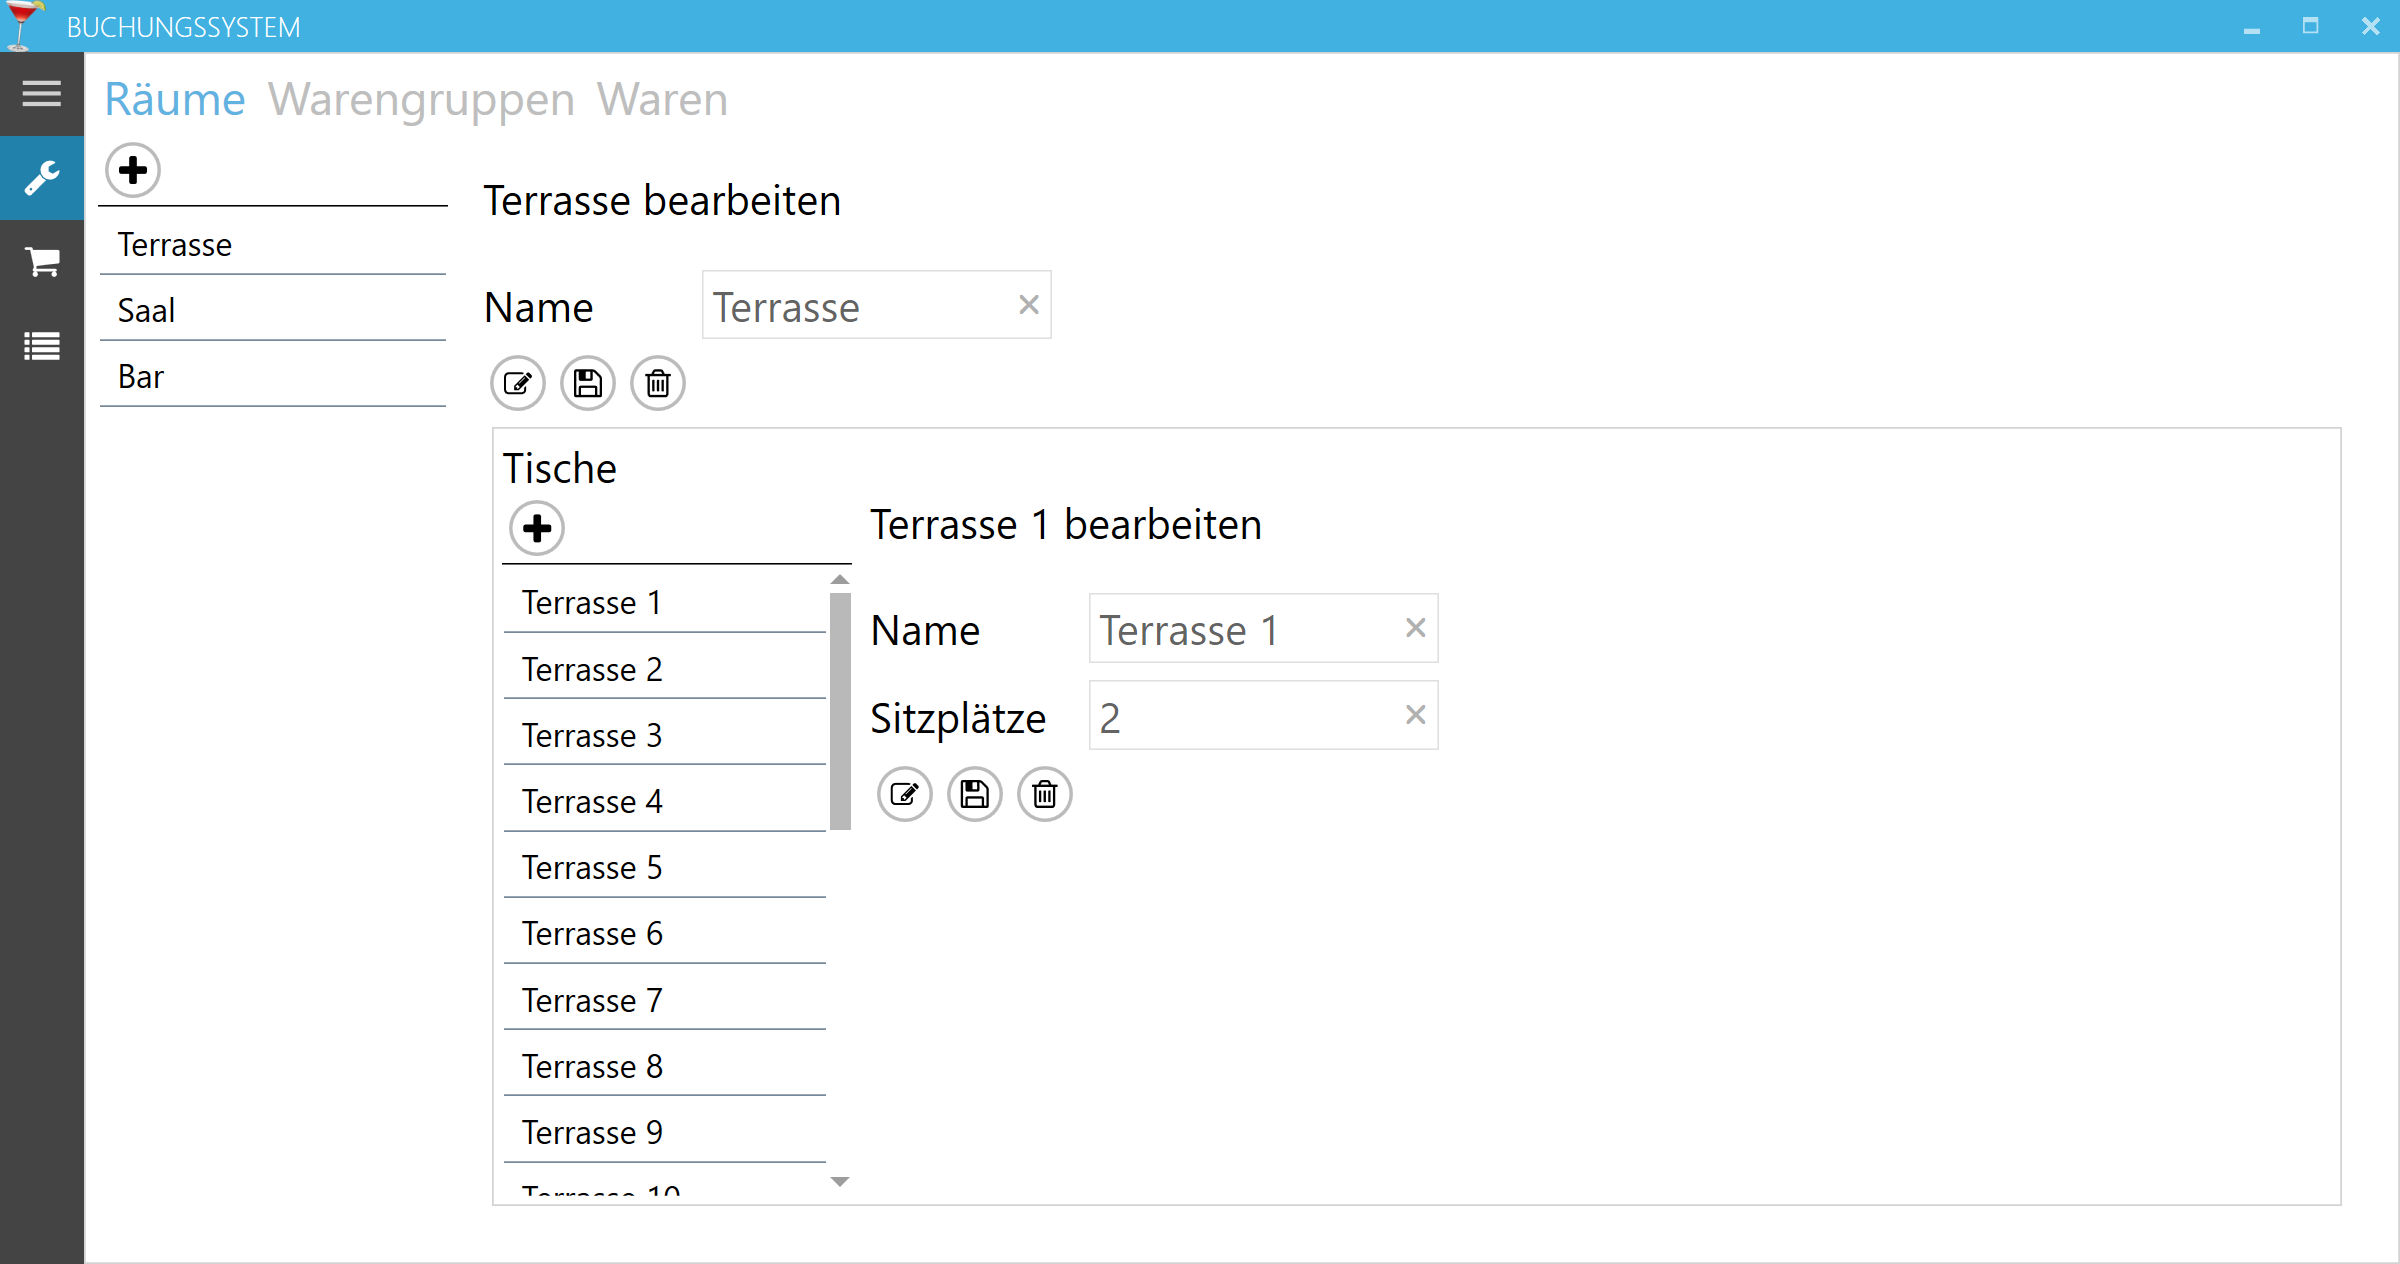
\includegraphics[width=\columnwidth]{Benutzerhandbuch/Raumverwaltung.png}
	\end{center}
	\caption{Übersicht der Raumverwaltung}
	\label{fig:room-management}
\end{figure}

\subsubsection{Warengruppen bearbeiten}

Um die Oberfläche für die Warengruppen aufzurufen, klicken sie in der Stammdatenverwaltung oben auf den Tab Warengruppen. Auf der linken Seite sehen sie eine Liste mit allen definierten Warengruppen. 

Wenn sie eine neue Warengruppe anlegen möchten, klicken sie auf den Plus-Button über der Warengruppenliste. 
Nun öffnet sie das Eingabeformular. Hier müssen sie einen Namen vergeben, sowie die übergeordnete Warengruppe angeben. 
So können sie eine Baumstruktur von Warengruppen erzeugen. 
Soll ihre Warengruppe keine Übergruppe haben, stellen sie den Schalter bei 'Keine Übergruppe' auf 'Ja'. Zum Abschluss klicken sie auf den Disketten-Button um die Warengruppe zu speichern.

Um eine Warengruppe zu Editieren, wählen sie in der Warengruppenliste eine Warengruppe aus. Öffnen sie die Editieransicht durch Klick auf den Editieren-Button.
Sie können den Namen sowie die Übergruppe ändern. Beachten sie, wenn sie die Übergruppe ändern, werden auch alle Waren, welche sich in der Warengruppe befinden, verschoben.

Um eine nicht mehr benötigte Warengruppe löschen, wählen sie in der Warengruppenliste eine Warengruppe an und klicken Sie auf den Mülltonnen-Button unter dem Eingabeformular.

\begin{figure}[h]
	\begin{center}
		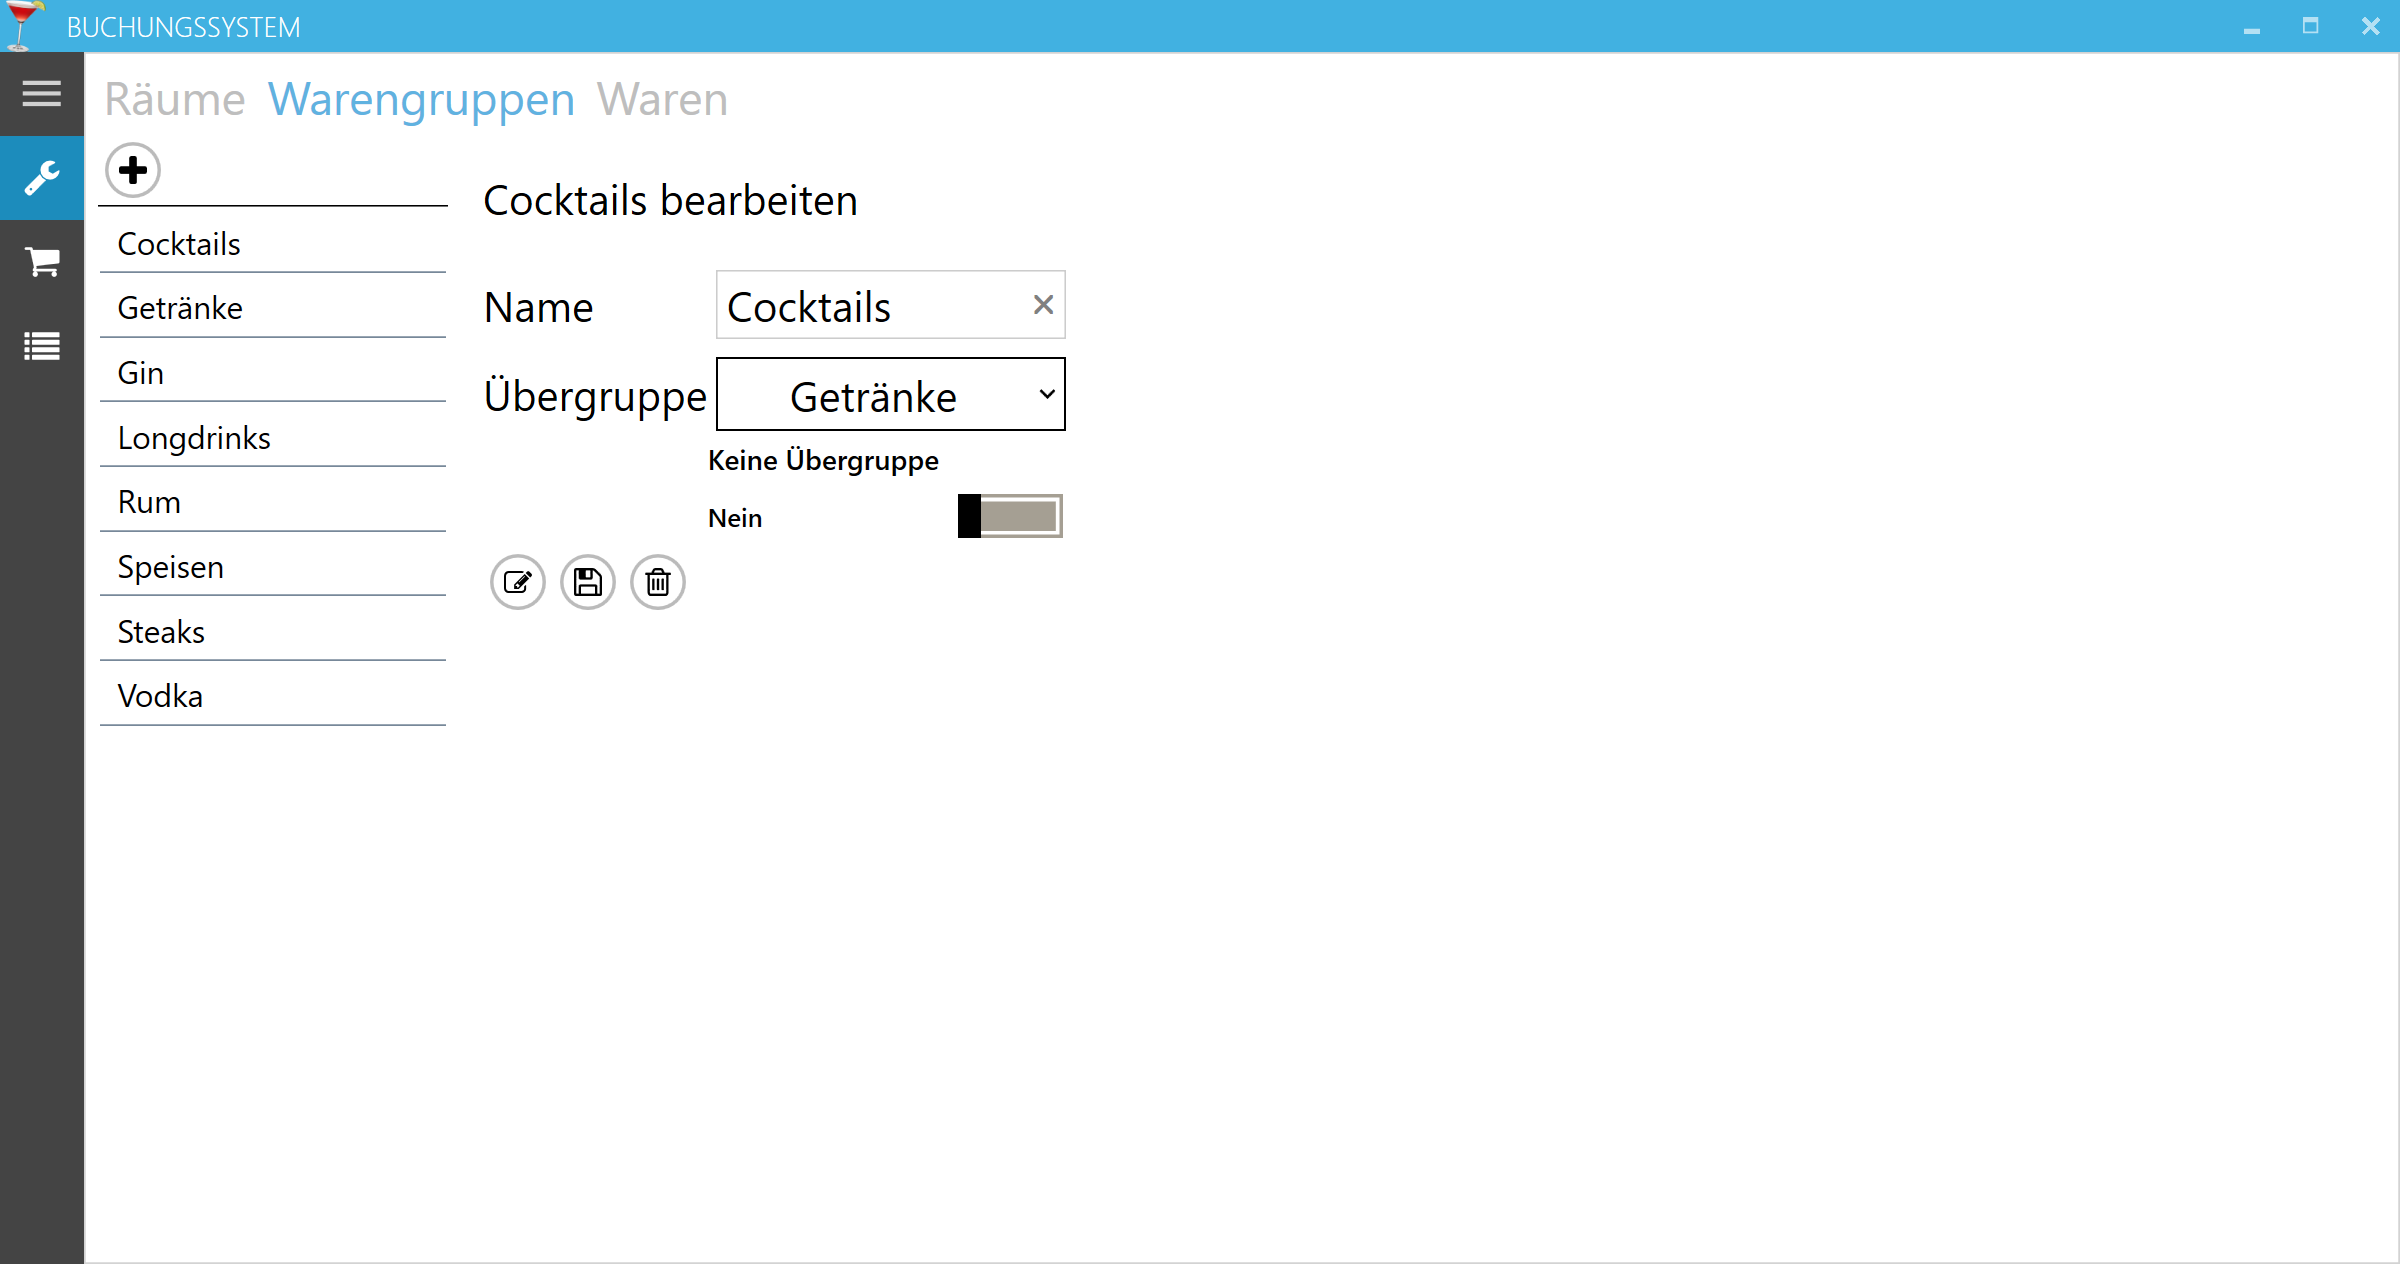
\includegraphics[width=\columnwidth]{Benutzerhandbuch/Warengruppenverwaltung.png}
	\end{center}
	\caption{Übersicht der Warengruppenverwaltung}
	\label{fig:productgroup-management}
\end{figure}

\subsubsection{Waren bearbeiten}

Um die Oberfläche für die Waren aufzurufen, klicken sie in der Stammdatenverwaltung oben auf den Tab Waren. Auf der linken Seite sehen sie eine Liste mit allen definierten Waren. 

Wenn sie eine Ware anlegen möchten, klicken sie auf den Plus-Button über der Warenliste. Nun öffnet sie das Eingabeformular. Hier müssen sie einen Namen vergeben,einen Preis, sowie die übergeordnete Warengruppe angeben. 
Sie können nur Warengruppen auswählen, die keine weiteren Warengruppen enthalten.
Zum Abschluss klicken sie auf den Disketten-Button um die Ware zu speichern.

Um eine Ware zu Editieren, wählen sie in der Warenliste eine Ware aus. Öffnen sie die Editieransicht durch Klick auf den Editiren-Button. 
Sie können den Namen, den Preis und die Übergruppe ändern.

Um eine nicht mehr benötigte Ware zu löschen, wählen sie in der Warenliste eine Ware aus und Klicken Sie auf den Mülltonnen-Button.

\begin{figure}[h]
	\begin{center}
		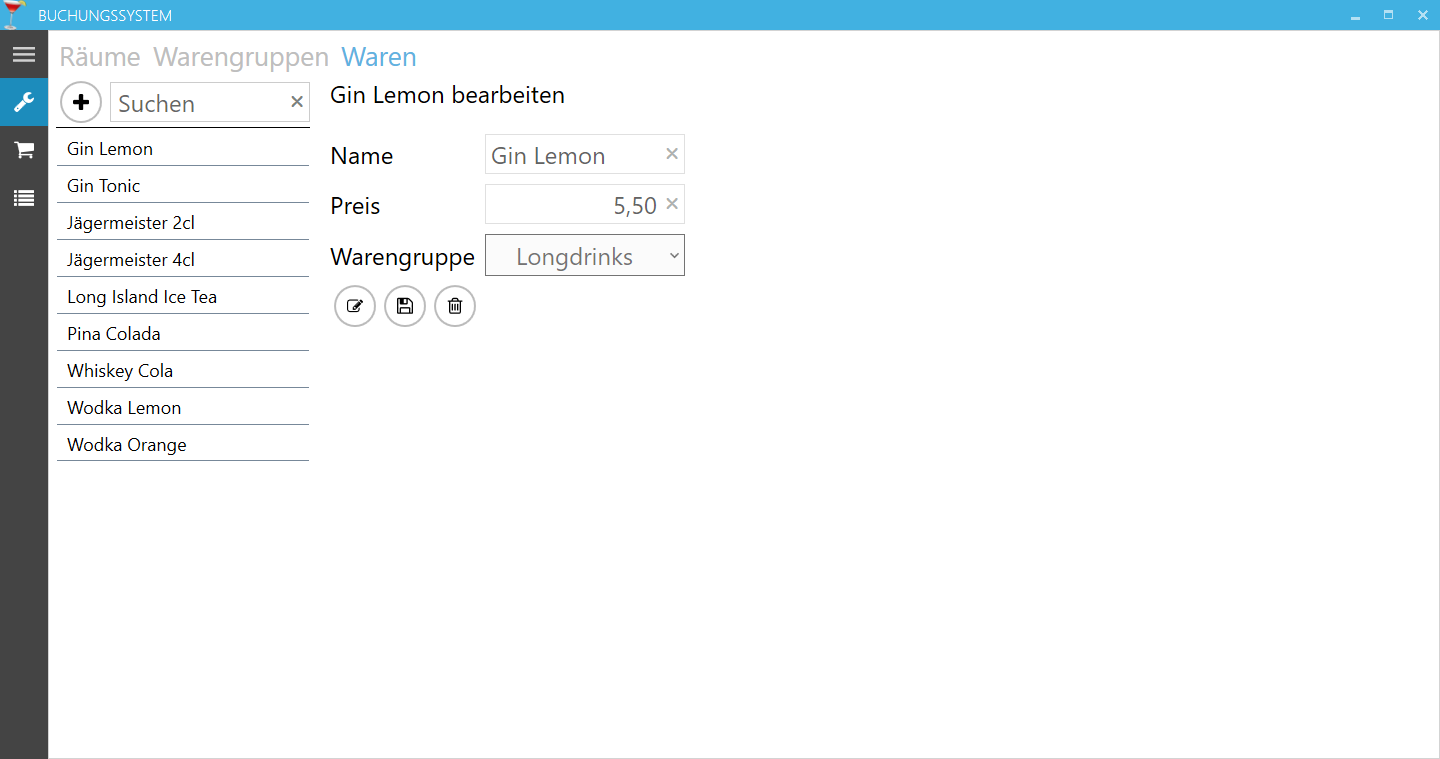
\includegraphics[width=\columnwidth]{Benutzerhandbuch/Warenverwaltung.png}
	\end{center}
	\caption{Übersicht der Warenverwaltung}
	\label{fig:product-management}
\end{figure}

\subsection{Buchungsverwaltung}

\subsection{Die Buchungsverwaltung aufrufen}

Die Buchungsverwaltung rufen Sie auf, indem Sie im Menü auf der linken Seite auf das Einkaufswagen-Symbol klicken. Alternativ können sie auch das Menu ausklappen. Nun erscheint neben den Symbolen auch die Beschriftung.
Die Buchungsverwaltung öffnet sich automatisch beim Start des Programmes. 
Hier finden Sie eine Übersicht aller Räume mit deren Tischen. In der Fußzeile sehen sie, wie viele Tische, und Plätze in dem ausgewähltem Raum Frei sind.

\begin{figure}[h]
	\begin{center}
		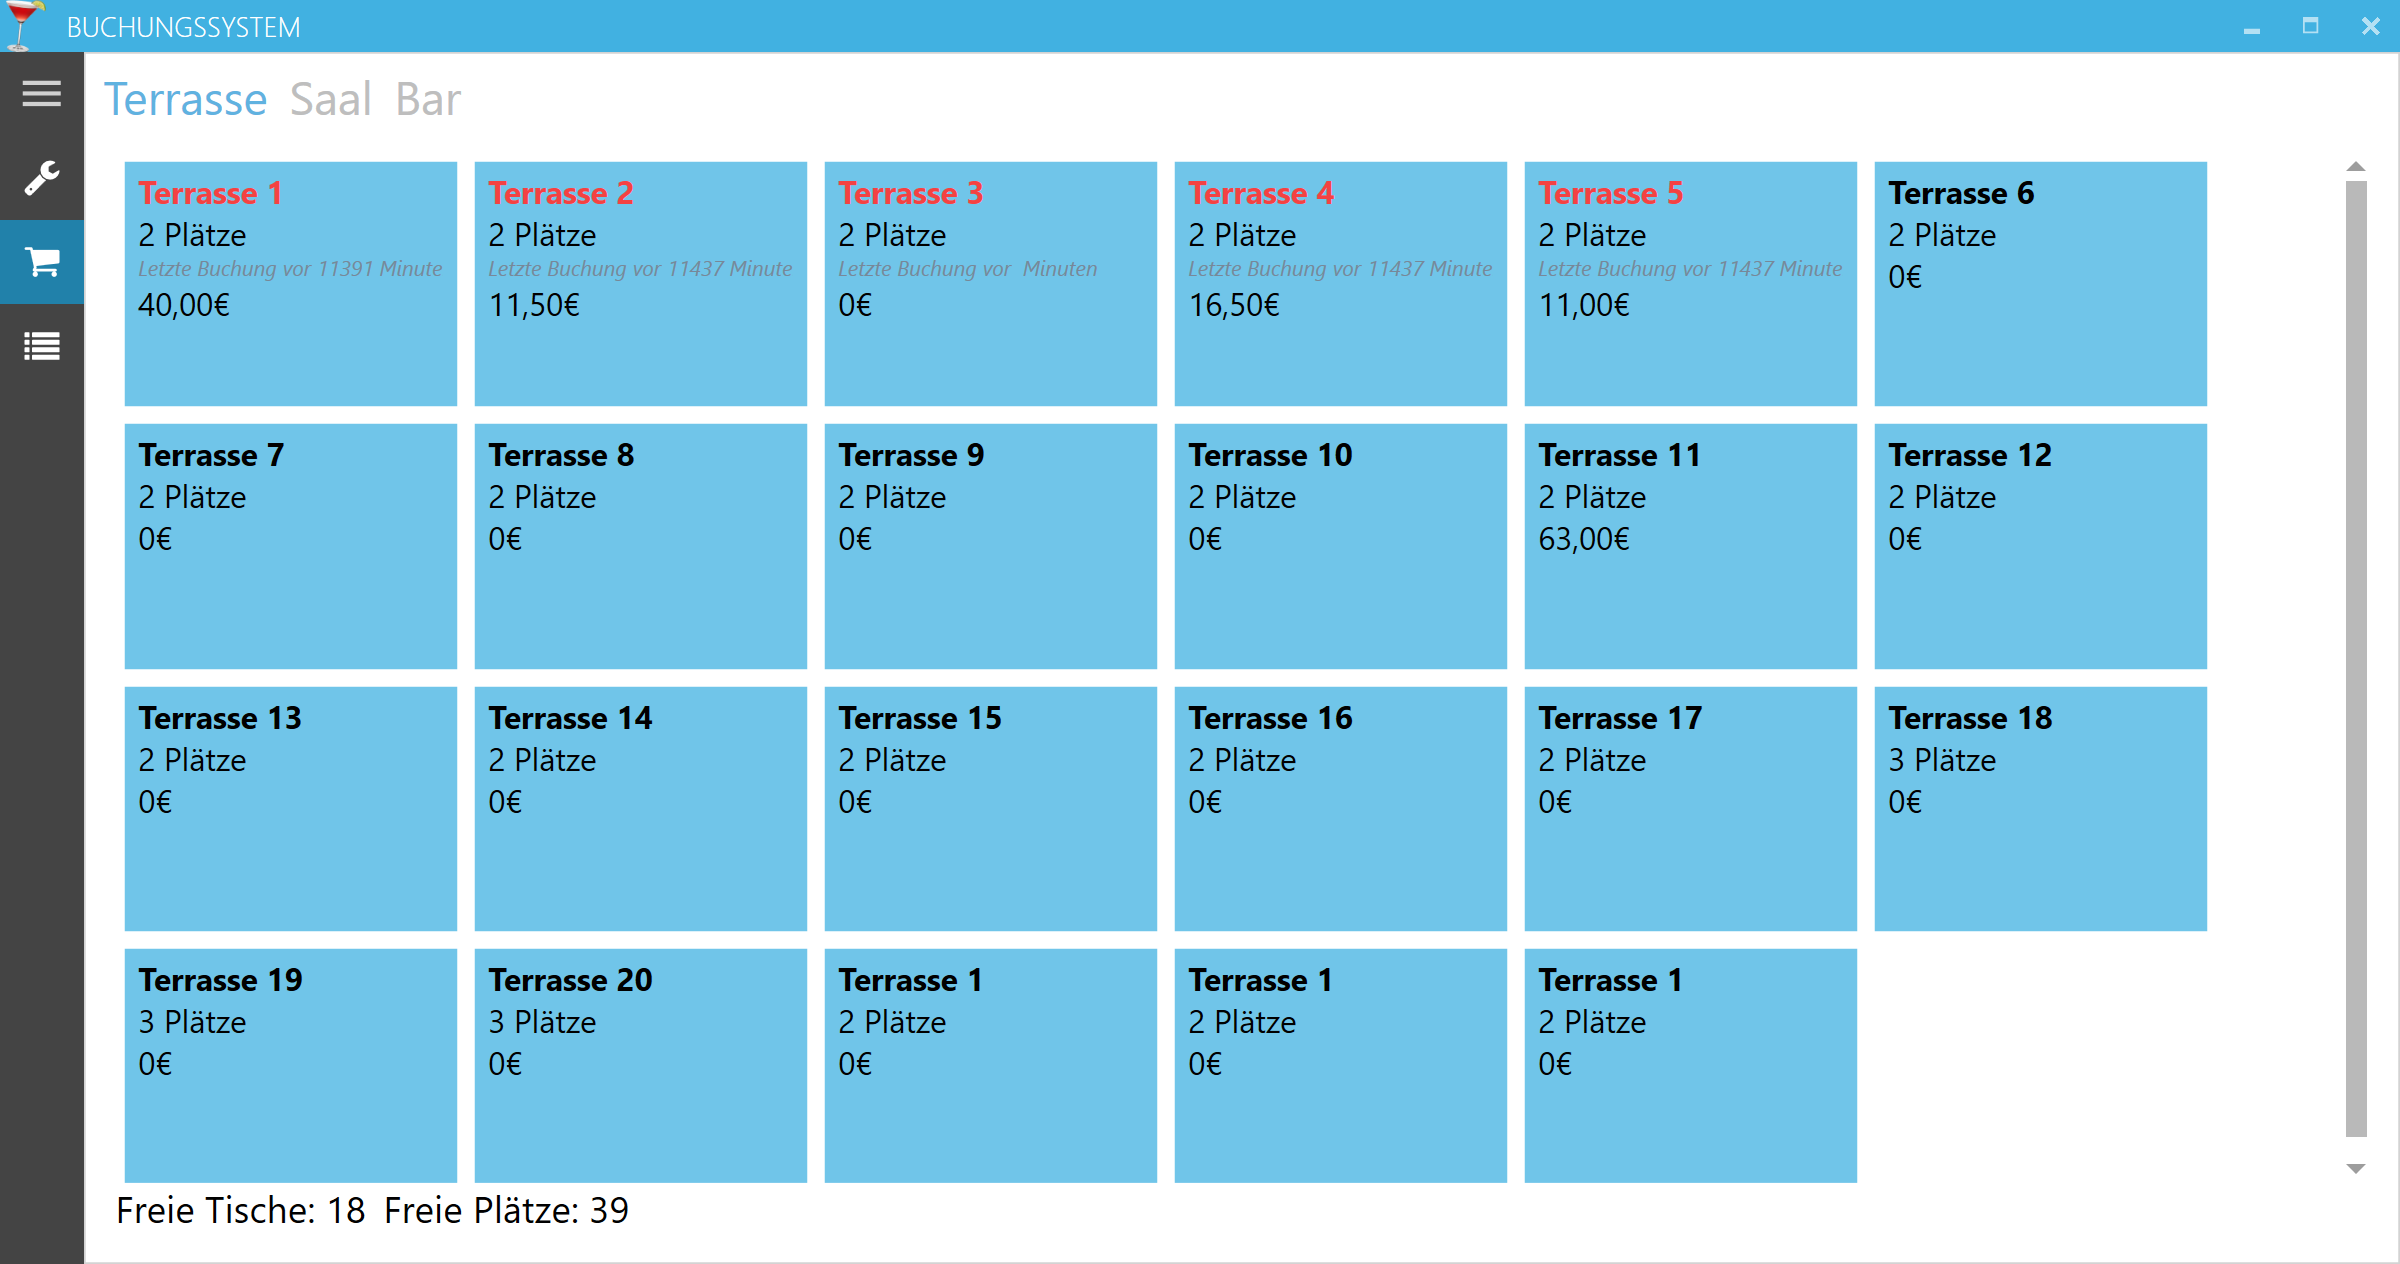
\includegraphics[width=\columnwidth]{Benutzerhandbuch/Tischuebersicht.png}
	\end{center}
	\caption{Raumübersicht}
	\label{fig:room-overview}
\end{figure}


\subsection{Status eines Tisches ändern}

Um einen Tisch zu besetzen, klicken sie mit der rechten Maustaste (bei einem Touch-Gerät alternativ lang mit dem Finger) um das Kontext-Menü zu öffen. Klicken Sie nun auf 'Status Ändern'. 
Der Tisch wird nun als Besetzt markiert. Auf die gleiche Weise machen Sie die Rückgangig.

\subsubsection{Ein Ware auswählen und Buchen}

Wählen durch Klick einen Tische an um die Tischübersicht zu sehen. Im linken Teil sehen sie die Warenauswahl. Im rechten die Buchungen auf diesem Tisch. 
Wählen sie in der linken Liste durch Klick eine Ware aus. Sie können beliebig viele Waren auswählen. Diese werden in einer Liste daneben zwischengespeichert. Um eine Ware zu deselektieren, klicken sie in der Liste der Ausgewählten Waren auf diese.
Um die ausgewählten Waren zu Buchen, klicken sie auf den 'Buchen'-Button unten links. Nun erscheint in der Liste der Buchungen für jede Ware eine Buchung.

In der Fußzeile der Buchungen sehen die den Gesamtbetrag, welcher auf dem Tisch gebucht ist.

\subsubsection{Buchungen als Bezahlt oder Storniert markieren}

Um Buchungen abzuschließen, wählen sie in der Tischübersicht eine oder mehrere Buchungen durch einen Klick auf diese aus. Diese werden dann in die Liste 'Ausgewählte Buchungen verschoben'. Diese können sie wiederum durch Klick darauf deselektieren.
Unter dieser Liste wird der Gesamtbetrag der ausgewählten Buchungen angezeigt. Klicken sie zum Schluss auf den Button 'bezahlen' um die Buchungen zu Bezahlen oder auf 'Stornieren' um die Buchungen zu Stornieren.

\begin{figure}[h]
	\begin{center}
		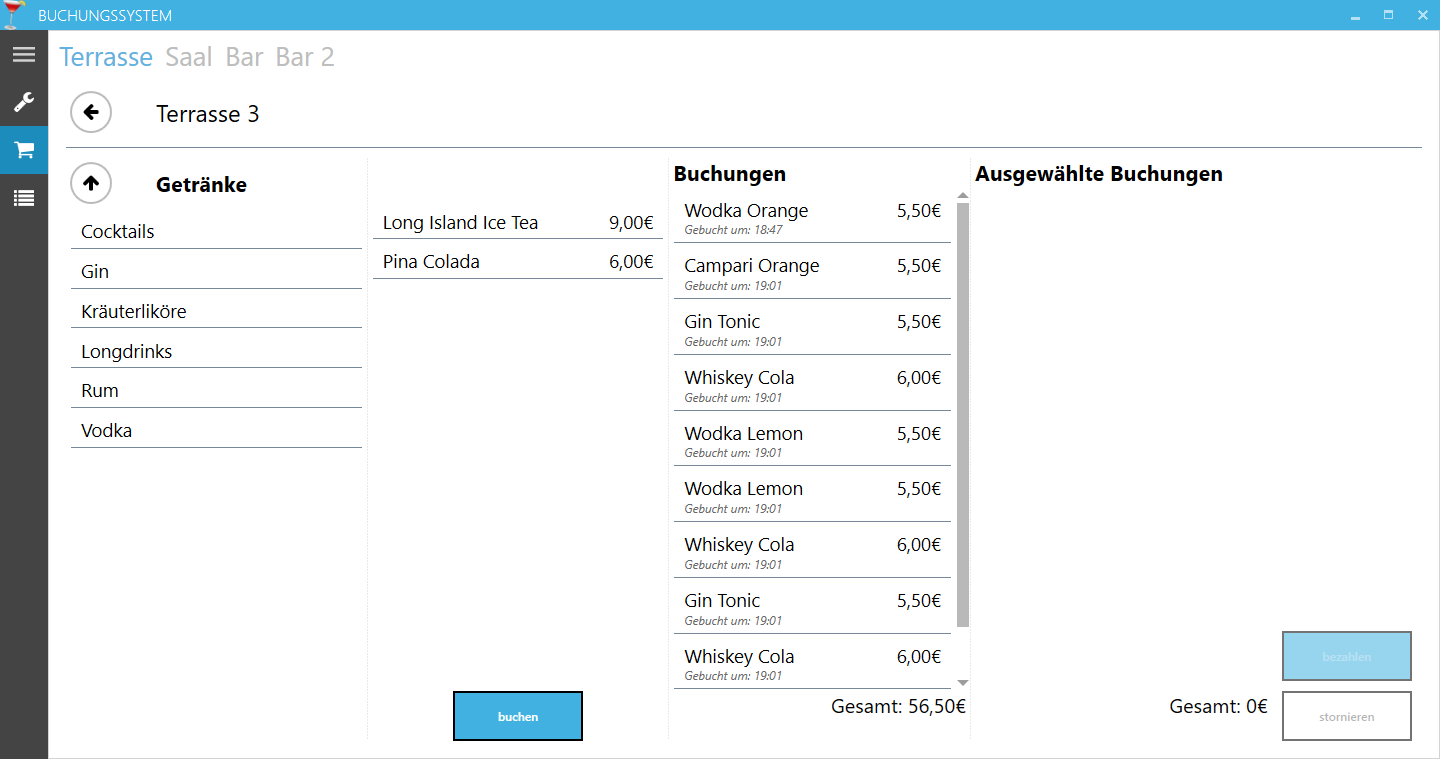
\includegraphics[width=\columnwidth]{Benutzerhandbuch/Buchungen.png}
	\end{center}
	\caption{Tischübersicht}
	\label{fig:table-overview}
\end{figure}

\subsection{Tagesübersicht}

Die Tagesübersicht rufen Sie auf, indem Sie im Menü auf der linken Seite auf das Listen-Symbol klicken. Alternativ können sie auch das Menu ausklappen. Nun erscheint neben den Symbolen auch die Beschriftung.

Hier können sie durch klicken auf den Kalender ein Datum auswählen. Haben Sie ein Daten ausgewählt, werden alle Buchungen von diesem Tag angezeigt. In der Fußzeile ist der Tagesumsatz zu sehen.
Beachten Sie, dass Offene und Stornierte Buchungen nicht in den Tagesumsatz fließen.